% Morley's theorem; triangle angles 62.10, 46.74, 71.16 degrees; Morley side 0.807014 = 8R sin(A/3)sin(B/3)sin(C/3).
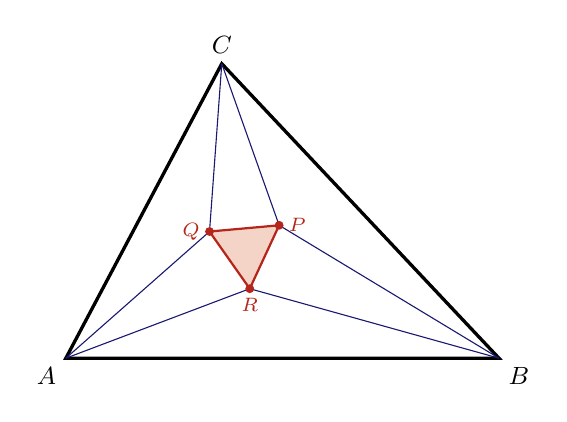
\begin{tikzpicture}[font=\small]
\draw[very thick] (0.0000,0.0000) -- (5.5000,0.0000) -- (1.9800,3.7400) -- cycle;
\draw[MidnightBlue] (0.0000,0.0000) -- (1.8243,1.6085);
\draw[MidnightBlue] (0.0000,0.0000) -- (2.3351,0.8824);
\draw[MidnightBlue] (5.5000,0.0000) -- (2.7085,1.6877);
\draw[MidnightBlue] (5.5000,0.0000) -- (2.3351,0.8824);
\draw[MidnightBlue] (1.9800,3.7400) -- (2.7085,1.6877);
\draw[MidnightBlue] (1.9800,3.7400) -- (1.8243,1.6085);
\draw[BrickRed,thick,fill=BrickRed!15] (2.7085,1.6877) -- (1.8243,1.6085) -- (2.3351,0.8824) -- cycle;
\fill[BrickRed] (2.7085,1.6877) circle (1.6pt) node[right,BrickRed,font=\scriptsize] {$P$};
\fill[BrickRed] (1.8243,1.6085) circle (1.6pt) node[left,BrickRed,font=\scriptsize] {$Q$};
\fill[BrickRed] (2.3351,0.8824) circle (1.6pt) node[below,BrickRed,font=\scriptsize] {$R$};
\node[below left] at (0.0000,0.0000) {$A$};
\node[below right] at (5.5000,0.0000) {$B$};
\node[above] at (1.9800,3.7400) {$C$};
\end{tikzpicture}
